\documentclass[a4paper]{article}


% Title Page


\usepackage{url}
\usepackage{amsmath}%
\usepackage{amsfonts}%
\usepackage{amssymb}%
\usepackage{mathtools}
\usepackage{bm}%
\usepackage{graphicx}
\usepackage{subfig}
\usepackage{cite}
\usepackage{sidecap}
\usepackage{fullpage}
\usepackage[a4paper,vmargin={20mm,20mm},hmargin={20mm,10mm}]{geometry}
\newcounter{mytempeqncnt}
\usepackage[T1]{fontenc}                


\newcounter{thcounter}
\newcounter{ascounter}
\newcounter{thcountera}
\newcounter{ascountera}
\newcounter{thcounterb}
\newcounter{ascounterb}

%\newenvironment{example}[1][Example]{\textbf{#1} }{ $\square$}

\DeclarePairedDelimiter\ceil{\lceil}{\rceil}
\DeclarePairedDelimiter\floor{\lfloor}{\rfloor}


\newenvironment{exercise}{
	\bigskip\noindent
	\refstepcounter{thcounter}
	\textbf{Problem \thethcounter}
}

\newenvironment{addexercise}{
	\bigskip\noindent
	\textbf{Additional problem}}

\newenvironment{assignment}{
	\bigskip\noindent
	\refstepcounter{ascounter}
	\textbf{Matlab assignment 1}
}


\font\myfont=cmr12 at 33pt


\title{Homework assignment 1}
\date{Lecturer: Duarte Antunes}
\author{Optimal control and dynamic programming (4SC000), TU/e, 2016-2017}
\begin{document}
	%\maketitle
	\thispagestyle{empty}
	\noindent	\hrulefill
	
	\textbf{Answer sheet homework 3}, 4SC000, TU/e, 2018-2019
	\begin{flushright}
		answer to problem 4 (1/3)
	\end{flushright}
	\noindent	\hrulefill
	$$(p(0),v(0))=(8,0)$$
				$$T=3.142$$
	\begin{itemize}
		\item[] Optimal input $u(t)$, postion $x(t)$ and velocity $v(t)$ with $t \in [0,T]$:
		\begin{figure}[h!]
			\centering
			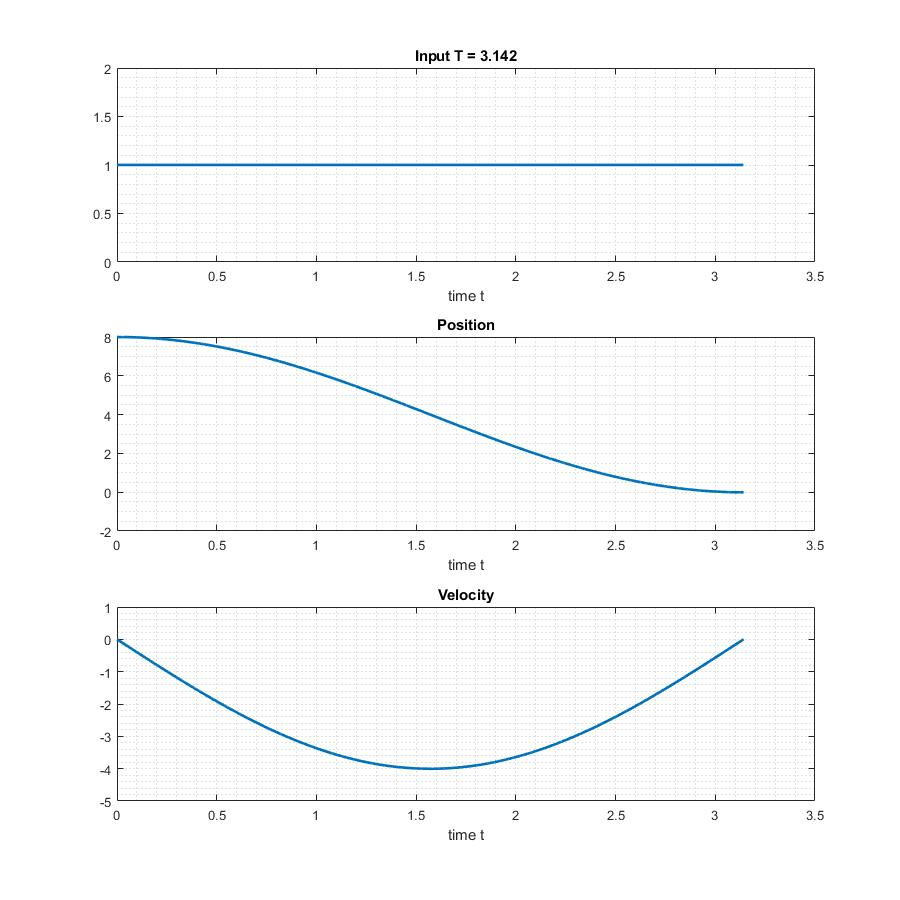
\includegraphics[width=9.5cm]{Solution_init1}
		\end{figure}
		\item[] State space plot position $x(t)$ and velocity $v(t)$:
		\begin{figure}[h!]
			\centering
			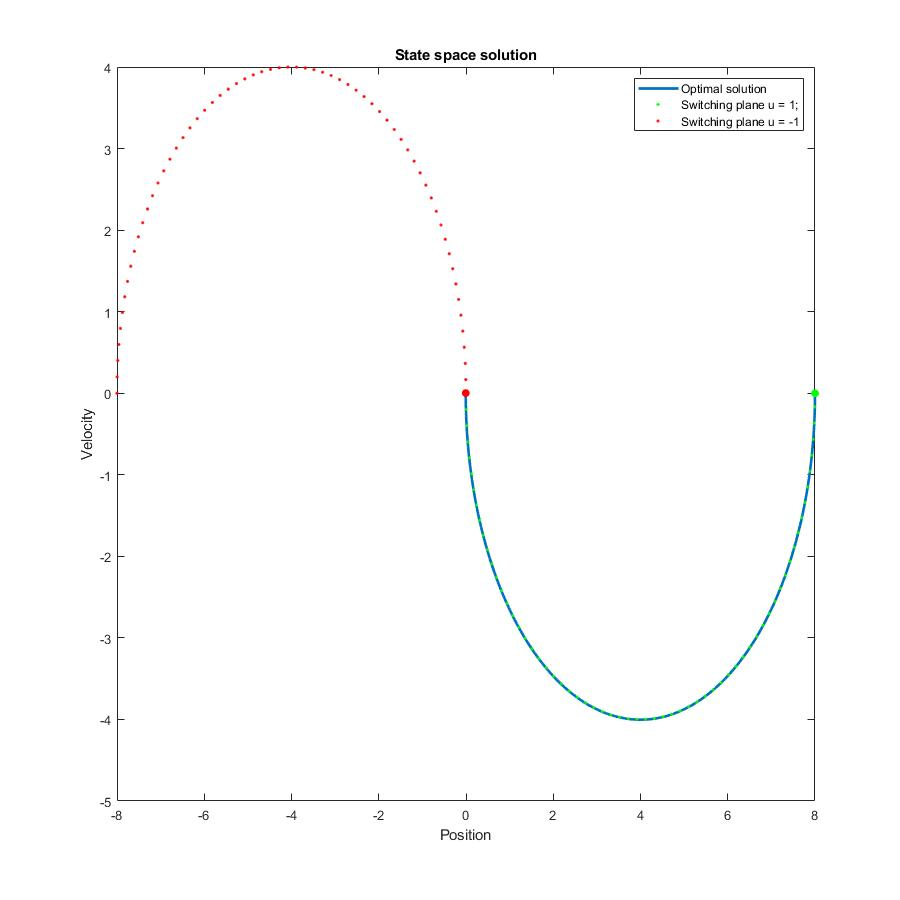
\includegraphics[width=9.5cm]{Statespace_init1}
		\end{figure}
	\end{itemize}
				
	\newpage
	\thispagestyle{empty}
	\noindent	\hrulefill
	\begin{flushright}
		answer to problem 4 (2/3)
	\end{flushright}
	\noindent	\hrulefill
	$$(p(0),v(0))=(-9,-8)$$
	$$T=5.21$$
	\begin{itemize}
		\item[] Optimal input $u(t)$, postion $x(t)$ and velocity $v(t)$ with $t \in [0,T]$:
		\begin{figure}[h!]
			\centering
			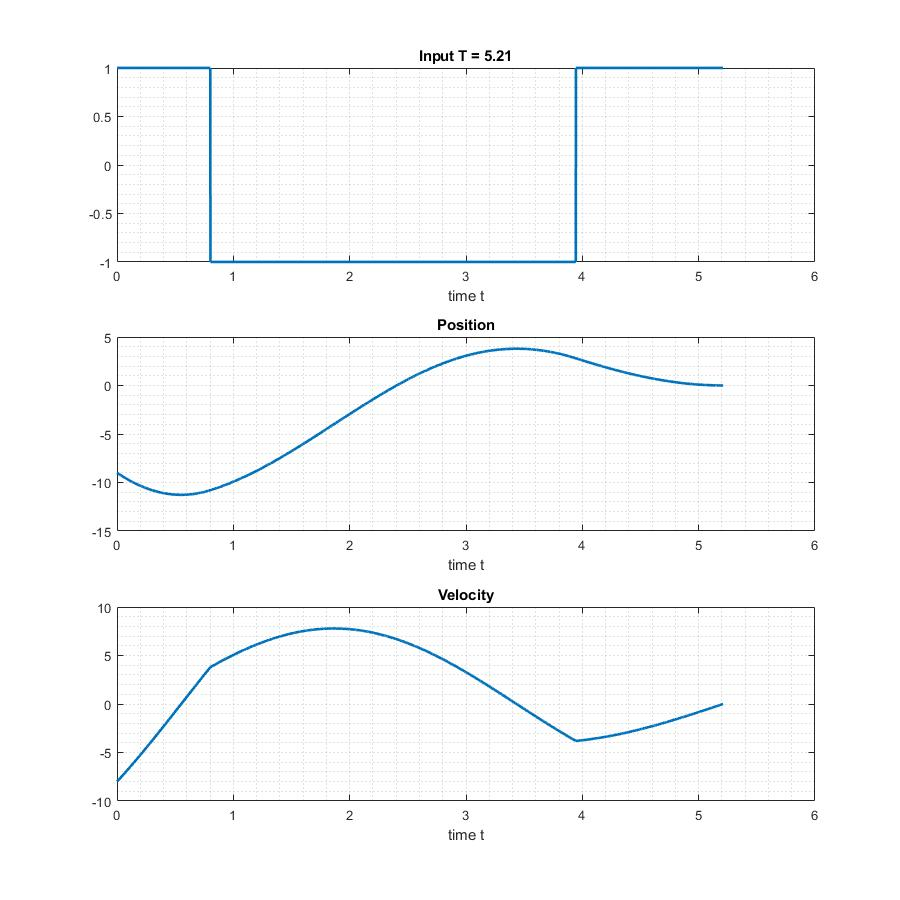
\includegraphics[width=9.5cm]{Solution_init2}
		\end{figure}
		\item[] State space plot position $x(t)$ and velocity $v(t)$:
		\begin{figure}[h!]
			\centering
			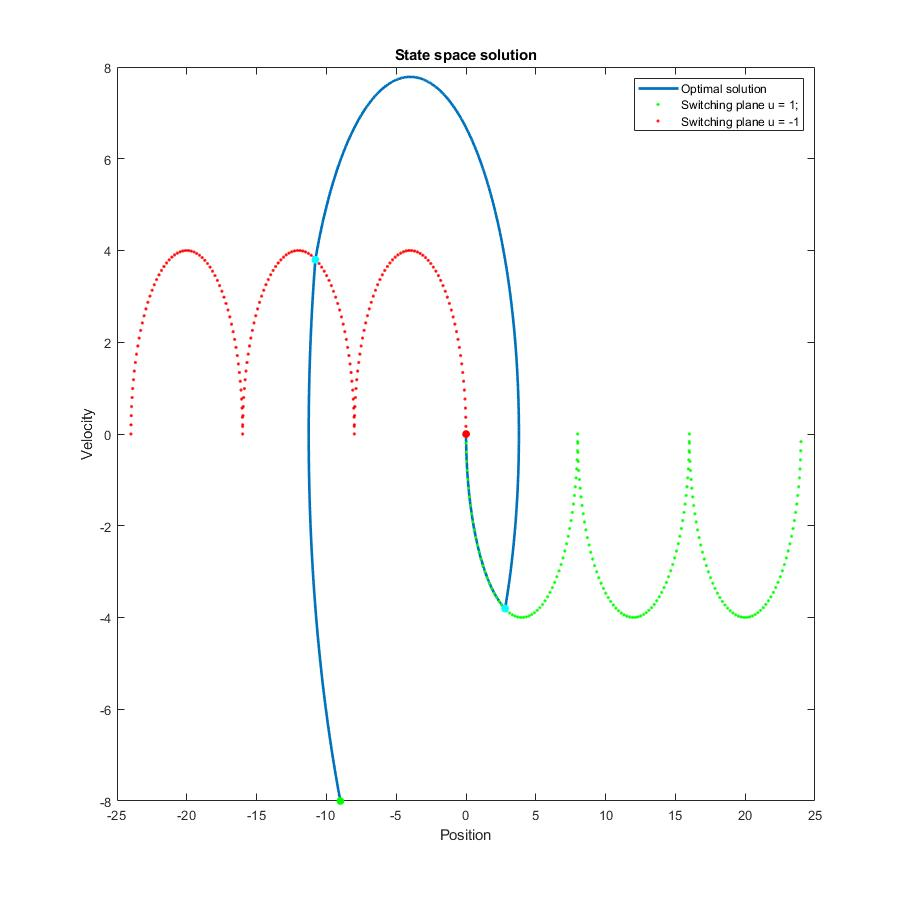
\includegraphics[width=9.5cm]{Statespace_init2}
		\end{figure}
	\end{itemize}
	\newpage
	\thispagestyle{empty}
	\noindent	\hrulefill
	\begin{flushright}
		answer to problem 4  (3/3)
	\end{flushright}
	\noindent	\hrulefill
	 $$(p(0),v(0))=(2,-1)$$
	 $$T=1.177$$
	\begin{itemize}
		\item[] Optimal input $u(t)$, postion $x(t)$ and velocity $v(t)$ with $t \in [0,T]$:
		\begin{figure}[h!]
			\centering
			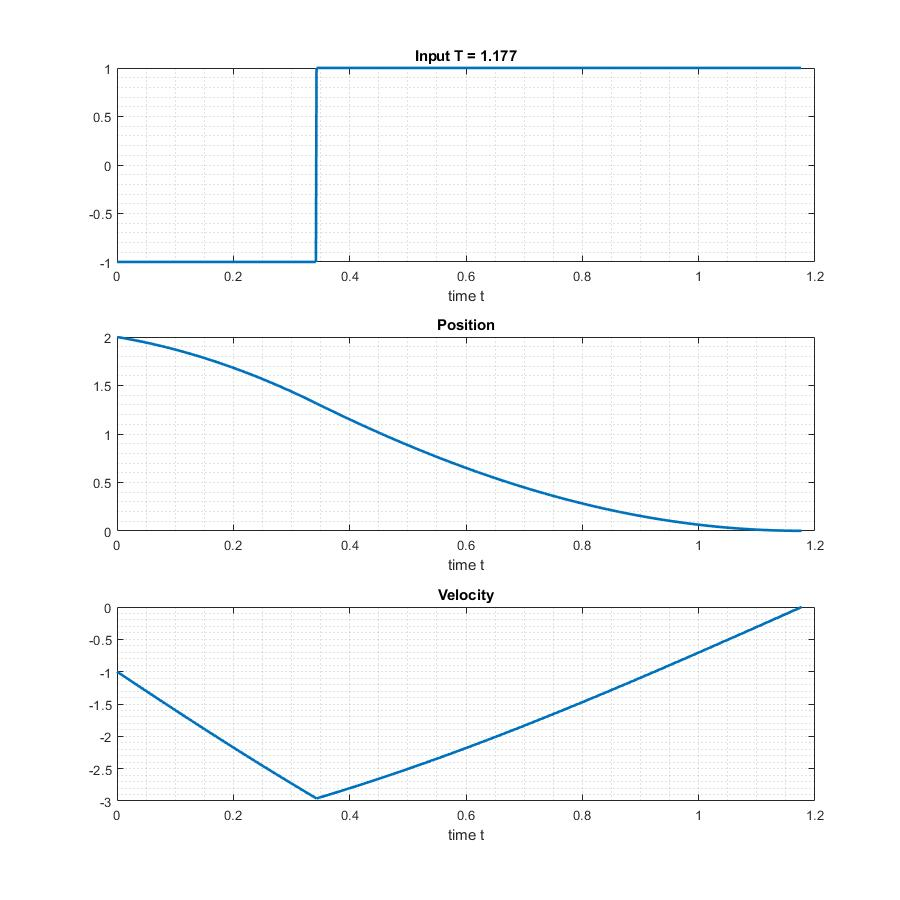
\includegraphics[width=9.5cm]{Solution_init3}
		\end{figure}
		\item[] State space plot position $x(t)$ and velocity $v(t)$:
		\begin{figure}[h!]
			\centering
			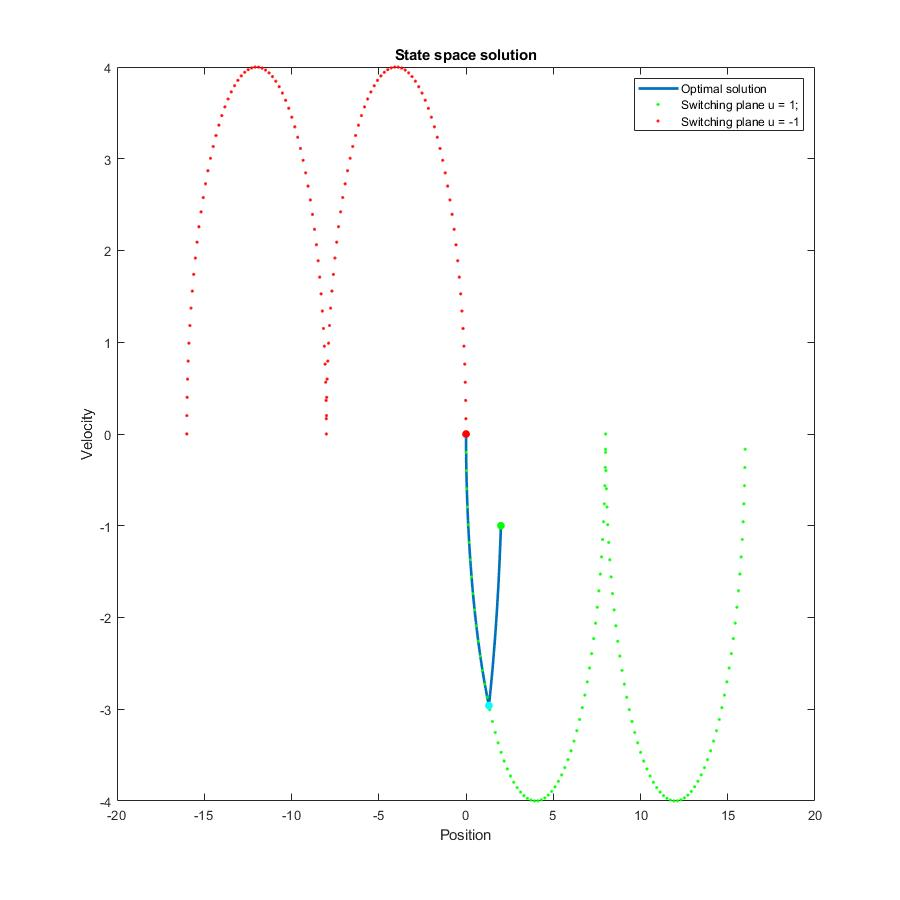
\includegraphics[width=9.5cm]{Statespace_init3}
		\end{figure}
	\end{itemize}
\end{document}
